\rhead{6. Klasni dijagram}
\section{Klasni dijagram}
\par Klasni dijagram je najvažniji dijagram za implementaciju. Zbog njegova važnosti, svaki deo klasnog dijagrama je opisan u nastavku.
Radi boljeg razumevanja, dijagram je podeljen na nekoliko segmenata:
\begin{itemize}
    \item Enumeracije
    \item Korisnici
    \item Zahtevi
    \item Donacija
    \item Objave
    \item Prevod dijagrama prelaza stanja, prethodno na dijagramu \ref{fig:state-class}
\end{itemize}
Čitav dijagram se može naći na dijagramu \ref{fig:class}.
\subsection{Enumeracije}
\par Enumeracije se koriste kada imamo tačan skup povezanih konstanti. Na klasnom dijagramu [Dijagram \ref{fig:enums}] se nalaze 4 enumeracije: 
\begin{itemize}
    \item TipPonude - koristi su klasi \textit{Ponuda} i ima vrednosti \textit{udomljavanje} i \textit{privremenSmeštaj}.
    \item TipNaloga - koristi se klasi \textit{KorisničkiNalog} i ima vrednosti \textit{administrator}, \textit{član} i \textit{volonter}.
    \item Pol - koristi se u klasi \textit{KorisničkiNalog} i ima vrednosti \textit{muško} i \textit{žensko}.
    \item Status - koristi se u klasama \textit{Ponuda} i \textit{Zahtev} i ima vrednosti \textit{prihvaćena}, \textit{odbijena} i \textit{naČekanju}.
\end{itemize}
\begin{figure}[h]
    \centering
    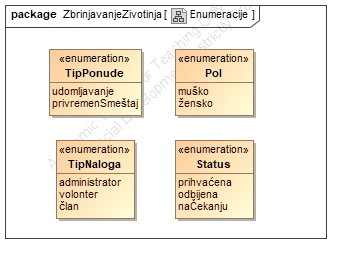
\includegraphics[width=0.5\textwidth, height=0.4\textwidth]{img/enums.jpg}
    \caption{Enumeracije u klasnom dijagramu}
    \label{fig:enums}
\end{figure}
\subsection{Korisnici}
\par Svaka \textit{osoba} ima \textit{KorisničkiNalog} i \textit{Adresa}.
Postoje dve naslednice klase \textit{Osoba} - \textit{Član} i \textit{Volonter}, koje nemaju dodatne atribute, ali zbog njihovih interakcija
sa drugim klasama, oni moraju da postoje u sistemu. Primetimo da ne postoje klase Gost i Administrator, jer oni nemaju dodatne interakcije
koje se razlikuju od prethodnih klasa. Svi \textit{koirnisčki nalozi} se pamte u klasi \textit{PetCentar}, kao i \textit{korisnički nalog} trenutno
ulogovane \textit{osobe}.
\par Korisnici u sistemu su prikazani na dijagramu \ref{fig:users}. 
\begin{figure}[h]
    \centering
    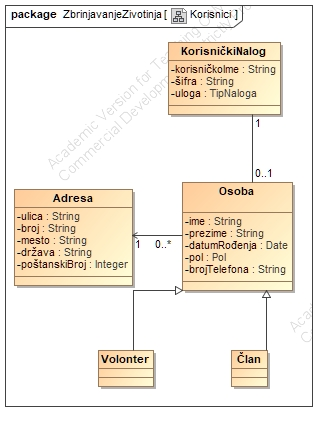
\includegraphics[width=0.5\textwidth, height=0.4\textwidth]{img/users.jpg}
    \caption{Korisnici u klasnom dijagramu}
    \label{fig:users}
\end{figure}
\subsection{Zahtevi}
\par Zahteve za promociju može samo da podnese \textit{član}, a da odobri \textit{volonter}. Ova interakcija je detaljnije prikazana 
na dijagramu sekvence [Dijagram \ref{fig:promotion-seq}]. Svi zahtevi se čuvaju u klasi \textit{PetCentar}.
\par Zahtevi su prikazani na dijagramu \ref{fig:reqs}.
\begin{figure}[h]
    \centering
    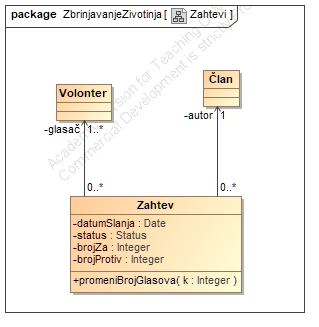
\includegraphics[width=0.5\textwidth, height=0.4\textwidth]{img/requests.jpg}
    \caption{Zahtevi u klasnom dijagramu}
    \label{fig:reqs}
\end{figure}
\subsection{Donacije}
\par Prijavljena \textit{osoba} može da donira. Pamti se ko je donirao kao i datum, dok se sve donacije pamte u klasi \textit{PetCentar}.
\par Donacije su prikazane na dijagramu \ref{fig:donations}.
\begin{figure}[h]
    \centering
    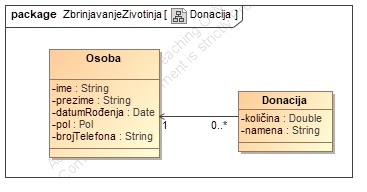
\includegraphics[width=0.5\textwidth, height=0.4\textwidth]{img/donation.jpg}
    \caption{Donacije u klasnom dijagramu}
    \label{fig:donations}
\end{figure}
\subsection{Objave}
\par Najbitniji deo klasnog dijagrama. Većina interakcija u sistemu su vezani za objave. Svaka objava sadrži \textit{komentare}, \textit{autora},
listu svih \textit{osoba} koji su označili objavu da im se sviđa, \textit{ponude}, \textit{životinju} za koju je vezana.
\par Ponude mogu da imaju \textit{recenziju}. 
\par Pored osnovnih informacija, \textit{životinja} sadrži i \textit{vrstu životinja}. Vrste životinja dodaje \textit{volonter}.
\par Objave su prikazane na dijagramu \ref{fig:posts}.
\begin{figure}[h]
    \centering
    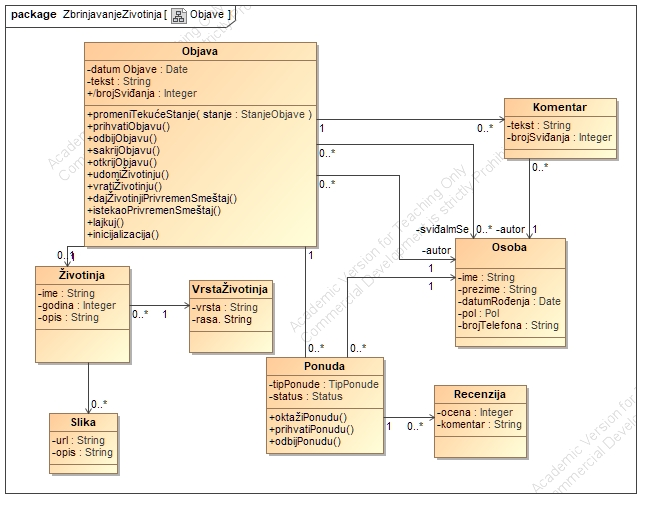
\includegraphics[width=\textwidth, height=0.55\textwidth]{img/posts.jpg}
    \caption{Objave u klasnom dijagramu}
    \label{fig:posts}
\end{figure}
\begin{sidewaysfigure}
    \centering
    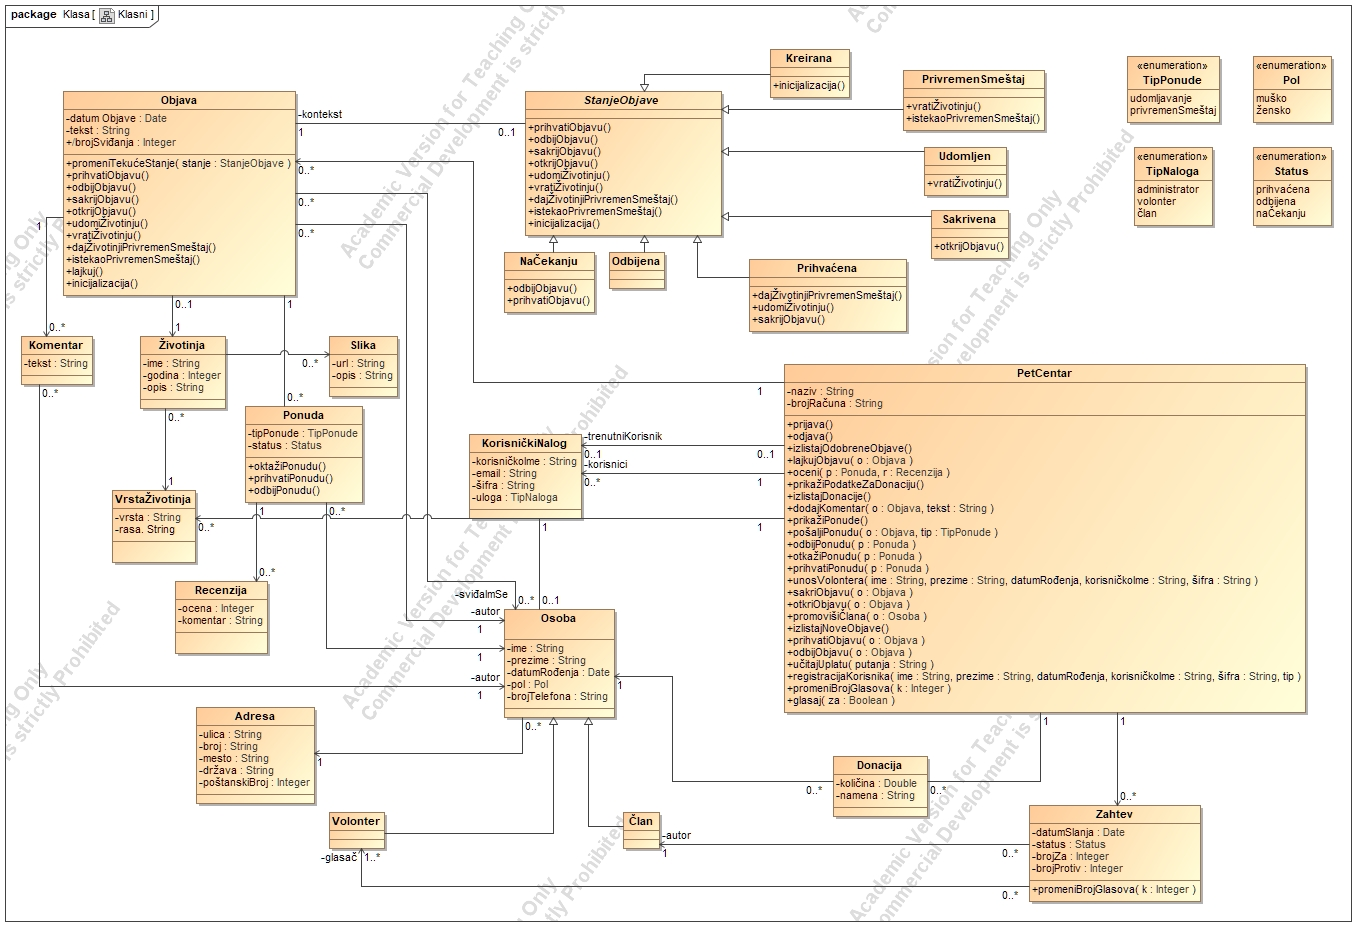
\includegraphics[width=\textwidth]{img/class.jpg}
    \caption{Klasni dijagram}
    \label{fig:class}
\end{sidewaysfigure}